\section{Setting up the embedded environment for software development}\label{zephyr}
PlatformIO is an open-source extension of Visual studio code, which supports hundreds of boards with different frameworks. \cite{Platform} Seeed XIAO nRF52840 is not natively suported. Seeed made library for Arduino IDE, which supports Arduino and Mbed framework, that was implemented through Github to PlatformIO and allows non-problematic implementation.
The XIAO has library in the Zephyr Github repository, but the PlatformIO does not use most recent version. The version of Zephyr itself is altered in PlatformIO and therefore does not work even after cross referencing with other boards already implemented in PlatformIO, such as Seeeduino (as a reference for the formfactor) or nRF52840 DK (as a reference for the chip).
The PlatformIO does not have inbuild serial USB communication, which results in inability to reprogram the board through the VS Code and need to go through bootloader first. This poses inconvinience, which can be avoided by use of a Arduino IDE, therefore if route of MBed or Arduino framework is chosen, Arduino IDE should be chosen. If the route of Zephyr is chosen, SDK by nordic semi is the optimal route, because event though it also does not have serial USB, it uses barebone Zephyr, as the Nordic Semiconductor SDK provides useful tools for development, such as build, flashing and debugging actions. \cite{nRF}

There is a caviat, profiles from GitHub of the current version of Zephyr via \path{Zephyr/boards/arm/xiao_ble} at main branch \cite{gitZephyr} can be used and imported the needed files into the SDK version of Zephyr we have.
In our case the path of the files would be in \path{~\ncs\v2.3.0-rc1\zephyr\boards\arm} .
After doing so, following the steps in the DevAcademy, nRF Connect SDK Fundamentals, Lesson 1 can be followed for setup. Then a blinky application can be created, and built via nRF Connect.
After a build of the application is created, a files for flashing will be created in the "build" subdirectory of the application.
To flash the Seeed XIAO nRF52840 Sense chip, entering a bootloader is needed, as it ships with the Adafruit nRF52 Bootloader, which supports UF2 flashing. \cite{docsZephyr}
Further more, a zephyr.ut2 file can be found in the "build" subdirectory of the application, after building the application, as we have done.
To access the bootloader, connect the Seeed XIAO to a PC.
Now to enter and flash an application, the reset button on the Seeed board should be clicked two times in quick succession, this will propmt the memory of the Seeed board on your PC.
Now find the previously mentioned zephyr.ut2 and drag it in to the memory of the Seeed board, and this will flash the board with the new application.

A issue accured when trying to test the "Hello World" application, when connecting to serial monitor no output is given.
After further investigation, it was noticed that the Seeed documentation, mentiones no debugging interface, hence no USB serial exists.
To solve the issue, an application called "console", from \path{zephyr/samples/subsys/usb/console} was cloned, in order to test a virtual USB serial connection, with the use of CDC ACM UART. \cite{gitZephyr}
After building and flashing, results were achieved. (See Figure~\ref{fig:serial})

\begin{figure}[H]
    \centering
    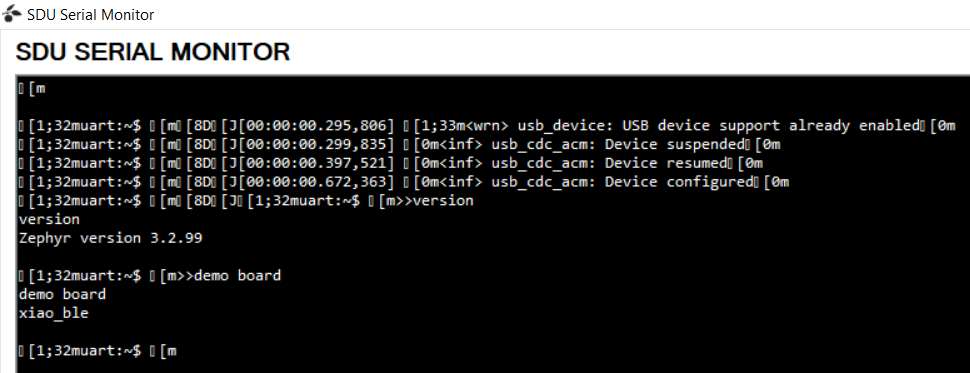
\includegraphics[scale = 0.7]{pictures/serial_monitor.png}
    \caption{Serial output of the XIAO MCU}
    \label{fig:serial}
\end{figure}

Another issue that arose was debugging. The Seeed XIAO nRF52840 Sense does not have any sort of built in debugging tools. \cite{wikiSeeed}
One can use a J-link debugging tool, but a caviet was found, which was GDB stub, which Zephyr supports, this would save budget. \cite{docsZephyr}
